
\chapter{Black-box TFNP} \label{chap:bb-tfnp}

\section{Oracles and decision trees}

In the previous chapter, we have discussed how \textsf{TFNP} subclasses are defined in terms of basic existence principles which can be converted into white-box total search problems solvable by protocols that are reducible to the Karchmer-Widgerson game. In this chapter, instead, we will extensively discuss the \textbf{black-box model}.

The difference between the white-box and black-box \textsf{TFNP} models can be formally described as the difference between problems verifiable (or computable) by a simple Turing machine or by a Turing machine equipped with an \textbf{oracle}. 

\begin{definition}
    An oracle for a problem $A$ is an external device that is capable of instantaneously verifying a solution for of such problem. An oracle Turing machine is a Turing machine provided with the ability of querying an oracle. We write $M^A$ to describe an oracle Turing machine provided with an oracle for the problem $A$.
\end{definition}

By definition, it's easy to see that an oracle is nothing more than a black-box device. In particular, an oracle for a decision problem is capable of determining if an input object has the the required property, while an oracle for a search problem is capable of determining if an output is the solution for the associated problem with the given input. Any query to the oracle made by the Turing machine has a complexity of $\Theta(1)$, meaning that it doesn't affect the cost of the computation. This allows us to give the following definition of query search problem \cite{proofs_circuits_communication, tfnp_characterization}.

\begin{definition}
    A query search problem is a sequence $R = (R_n)_{n \in \N}$ of relations $R_n \subseteq \{0,1\}^n \times O_n$, one for each $n \in \N$, where each $O_n$ is a finite set called "outcome set".
\end{definition}

Additionally, oracles provide a simple yet effective way to generalize the concept of reduction, called \textbf{Turing reductions}: if a Turing machine provided with an oracle for the problem $B$ is capable of resolving a problem $A$ then the problem $A$ can be reduced to the problem $B$. The idea behind this kind of reductions is simple: if $M^B$ can solve $A$ then any query to the oracle can be replaced with a call to a subroutine that solves $B$. Many-to-one reductions can be seen as restricted variants of Turing reductions where the number of calls made to the subroutine of problem $B$ is exactly one and the value returned by the reduction is the same value as the one returned by the subroutine.

More generally, given a class $\mathcal{C}$ and an oracle for a problem $A$, the \textit{relativized version} of the class $\mathcal{C}$ is the set of all problems of $\mathcal{C}$ verifiable (or solvable) with access to the oracle of $A$. Obviously, this definition implies that $\mathcal{C} \subseteq \mathcal{C}^A$ for all oracles $A$ since any problem that is already in $\mathcal{C}$ can just ignore the oracle. In the particular case of \textsf{TFNP}, it was proven that the relation between each total search problem is strictly connected to the relation of the relativized versions of their classes \cite{rel_comp_np_search}.

\begin{theorem}
    Given two search problems $R,S \in \mathsf{TFNP}$ and their relative classes it holds that $R \subseteq S$ if and only if $R^A \subseteq S^A$ for all oracles $A$.
\end{theorem}

This result states that proving any relativized separation is equivalent to proving a non-relativized separation, allowing us to use the intuitive nature of oracles to rule out possible collapses in \textsf{TFNP} subclasses. Through these relativized separations, many \textsf{TFNP} subclasses have been proven to be different.

Moreover, the use of oracles allows us to model total search problem through the lens of \textbf{decision trees}.

\begin{definition}[\cite{search_problems_dt_model}]
    A decision tree is a rooted directed binary tree whose nodes are associated with either an output value or an input Boolean variable. Each leaf is labeled with an output $o \in O$, where $O$ is the outcome set. Each internal node is labeled by a variable and the two outgoing edges are labeled by the two possible values of that variable.
\end{definition}

Decision trees can be viewed as nothing more than the \textit{black-box version} of protocols: we don't care about who computes the next step and how they do it, we only care about the result being either a 0 or a 1 in order to proceed with the computation. In fact, like their white-box counterpart, a decision tree encodes all possible ways to obtain a result, making them \textit{total}. Likewise, the complexity of a decision tree computing a function follows the same complexity measures as a protocol, i.e. its \textit{size} and its \textit{depth}.

\begin{figure}[H]
    \centering

    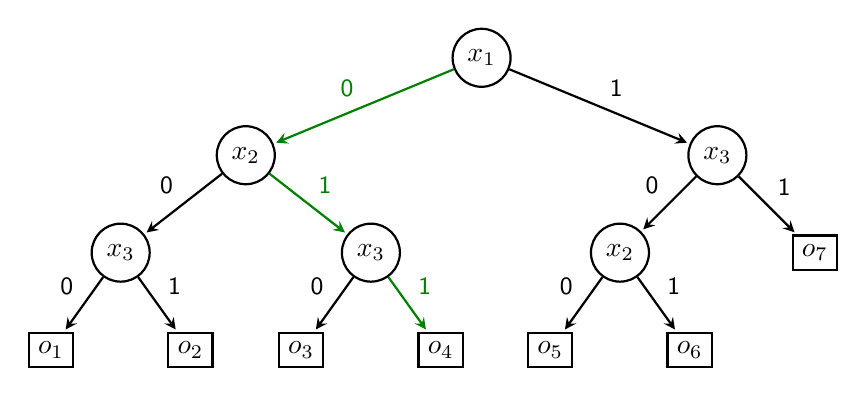
\begin{tikzpicture}[->,>=stealth,shorten >=1pt,auto,node distance=1.75cm, thick,main node/.style={scale=0.9,circle,draw,font=\sffamily\normalsize}]

        \node[circle, draw] (1)[] {$x_1$};

        \node[circle, draw] (2) [below left of=1, xshift=-50, ]{$x_2$};
        \node[circle, draw] (3) [below right of=1, xshift=50, ]{$x_3$};

        \node[circle, draw] (4) [below left of=2, xshift=-10, ]{$x_3$};
        \node[circle, draw] (5) [below right of=2, xshift=10, ]{$x_3$};
        \node[circle, draw] (6) [below left of=3, ]{$x_2$};
        \node[rectangle, draw] (7) [below right of=3]{$o_7$};

        \node[rectangle, draw] (8) [below left of=4, xshift=10]{$o_1$};
        \node[rectangle, draw] (9) [below right of=4, xshift=-10]{$o_2$};
        \node[rectangle, draw] (10) [below left of=5, xshift=10]{$o_3$};
        \node[rectangle, draw] (11) [below right of=5, xshift=-10]{$o_4$};
        \node[rectangle, draw] (12) [below left of=6, xshift=10]{$o_5$};
        \node[rectangle, draw] (13) [below right of=6, xshift=-10]{$o_6$};

        \path[every node/.style={font=\sffamily\small}]
            (1) edge[swap, color=Green]  node{0} (2)
            (1) edge node{1}(3)

            (2) edge[swap]  node{0} (4)
            (2) edge[color=Green]  node{1}(5)

            (3) edge[swap]  node{0} (6)
            (3) edge  node{1}(7)
            
            (4) edge[swap]  node{0} (8)
            (4) edge  node{1}(9)

            (5) edge[swap]  node{0} (10)
            (5) edge[color=Green]  node{1}(11)

            (6) edge[swap]  node{0} (12)
            (6) edge  node{1}(13)
        ;
    \end{tikzpicture}

    \caption{An example of decision tree of size 13 and depth 3. The computation, shown by the green path, for the input $x \in \{0,1\}^n$ is given by $x = 011$}
\end{figure}

Decision trees give an easier way to describe the computation of an oracle Turing machine: if $M^B$ verifies (or solves) a problem $A$ then the $i$-th query made by the procedure corresponds to a variable $x_i$ for the decision tree where $x_i = 1$ if the query returns a positive result and 0 otherwise. In other words, the computation tree of an oracle Turing machine is actually a decision tree.

\begin{proposition}
    If there is an oracle Turing machine $M^B$ that verifies (or solves) a problem $A$ then there is a decision tree that verifies (or solves) $A$. \unsure{Not sure if it's an if and only if, possibly yes}
\end{proposition}

The above proposition gives a strong result that allows us to characterize black-box \textsf{TFNP} through decision trees instead of oracles: \textit{any decision tree separation implies a relativized separation}. As in the communication complexity formulation described for the white-box model, given a \textsf{TFNP} problem $R$, we denote with $R^{dt}$ the equivalent \textsf{TFNP}$^{dt}$ problem, where \textit{dt} stands for \textit{decision tree} \cite{proofs_circuits_communication, tfnp_characterization}.

\begin{definition}
    We define $\mathsf{FP}^{dt}$ as the set of query search problems $R = (R_n)_{n \in \N}$ for which there exists a polylogarithmic depth decision tree $T_n$ such that $T_n(x) = y$ if and only if $(x,y) \in R_n$. Likewise, we define $\mathsf{FNP}^{dt}$ as the set of query search problems $R = (R_n)_{n \in \N}$ for which there exists a polylogarithmic depth decision tree $T_y$ such that $T_y(x) = \mathrm{True}$ if and only if $(x,y) \in R_n$.
\end{definition}

Furthermore, we also introduce the concept of decision tree reductions. Differently from classic and communication search problems, these reductions are based on a more fine-grained definition, where the function that maps inputs of the first problem to inputs of the second problem is computed by many decision trees with output $\{0,1\}$. This definition will allow us to prove some following results in a more convenient way. An analogous formulation can be obtained by computing this function through a simple decision tree. 

\begin{definition}
    A query search problem $R = (R_m)_{m \in \N}$, where $R_m \subseteq \{0,1\}^m \times O_m$ is said to be many-to-one reducible to a query search problem $S = (S_n)_{n \in \N}$, namely $R \leq S$, where $S_n \subseteq \{0,1\}^n \times O_n'$, if for all $m \in \N$ there is an $n \in \N$ for which there is a family of decision trees $T_i : \{0,1\}^m \to \{0,1\}$ for each $i \in [n]$ and a decision tree $T^y : \{0,1\}^m \to O_m$ for each $y \in O_n'$ such that:
    \[\forall x \in \{0,1\}^m \;\; (T(x), y) \in S \implies (x, T^y(x)) \in R\]
    where $T(x) := (T_1(x), \ldots, T_n(x))$. In other words, the decision trees $T_1, \ldots, T_n$ map inputs of $R$ into inputs of $S$, while the decision tree $g$ maps solutions of $S$ into solutions of $R$. 
\end{definition}

The difference in notation between $T_1, \ldots, T_n$ and $T^y$ underlines the fact that the former give a $\{0,1\}$ output, while the latter gives a more complex output.The \textit{size} $s$ of the reduction is the number of input bits to $S$, that being $n$. The \textit{depth} $d$ of the reduction is the maximum depth of any tree involved in the reduction, including both $T_1, \ldots, T_n$ and $T^y$. The \textbf{complexity of the reduction} is given by $\log s + d$. Moreover, we denote as $R^{dt}(S)$ the minimum complexity of any decision tree reduction from $R$ to $S$.

\newpage

Using this definition, we can define complexity classes of total query search problems via decision tree reductions: given a total query search problem $S = (S_n)_{n \in \N}$, we define the subclass of problems reducible to $S$ as:
\[S^{dt} := \{R : S^{dt}(R) = \mathrm{polylog}(n)\}\]
where $R = (R_m)_{n \in \N}$.

\section{Proof complexity characterization}

\section{(?) An in-depth example: \textsf{FP}$^{dt}$ and $\mathrm{TreeRes}$}

\cleardoublepage